\chapter{Finite Element Modeling}
\label{chap:FEM}

In this chapter, the development of the finite element model of the UBX metro and the simulation setup are described. First, in section \ref{section:geometry}, the design of the model geometry and the mesh of the model are shown. Then, in section \ref{section:boundary_conditions}, the incorporation of boundary conditions into the finite element model is described. Finally, in section \ref{section:parametric_study}, a parametric study is carried out to investigate the influence of different simulation parameters on the solution of the initial finite element model. All these simulations are done with the acoustics module of the open-source FEM software openCFS \cite{opencfs}.


\section{Geometry and mesh}
\label{section:geometry}

As shown in sec. \ref{section:ubx_geometry}
Due to the large dimension of the car body 

a representative model has to be

\begin{figure}[H]
	\centering
	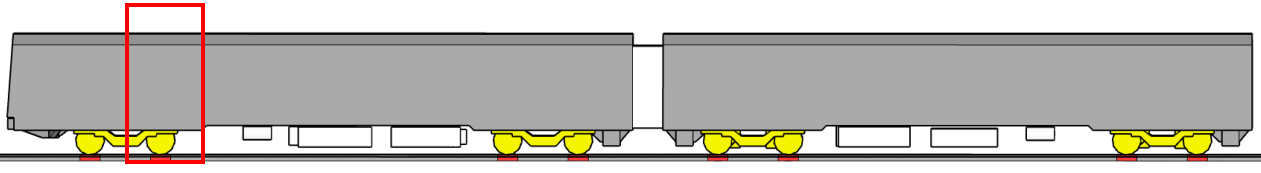
\includegraphics[width=\textwidth]{fig/chap4/geometry/model_area.png}
	\caption{Side view of UBX, red box marked the modeling area}
\end{figure}

\begin{figure}[H]
	\centering
	\begin{subfigure}[b]{0.4\textwidth}
		\centering
		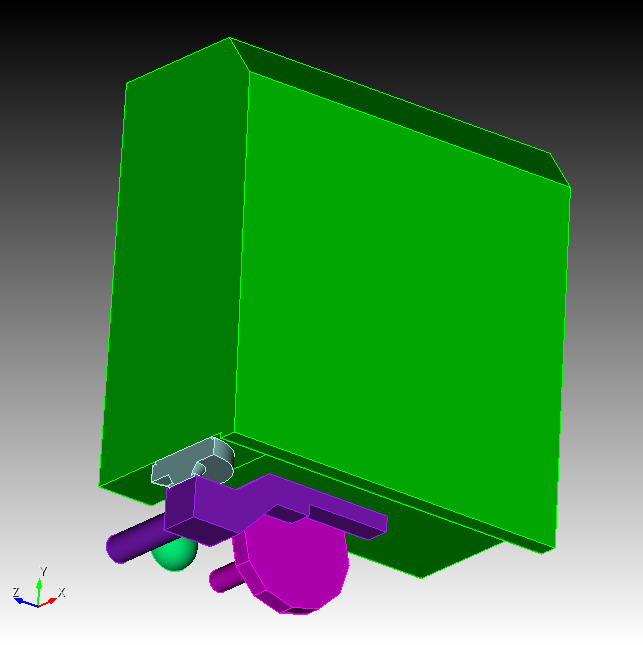
\includegraphics[width=0.9\linewidth]{fig/chap4/geometry/one_fourth_model.png}
		\caption{quarter model}
	\end{subfigure}
	\hfill
	\begin{subfigure}[b]{0.4\textwidth}
		\centering
		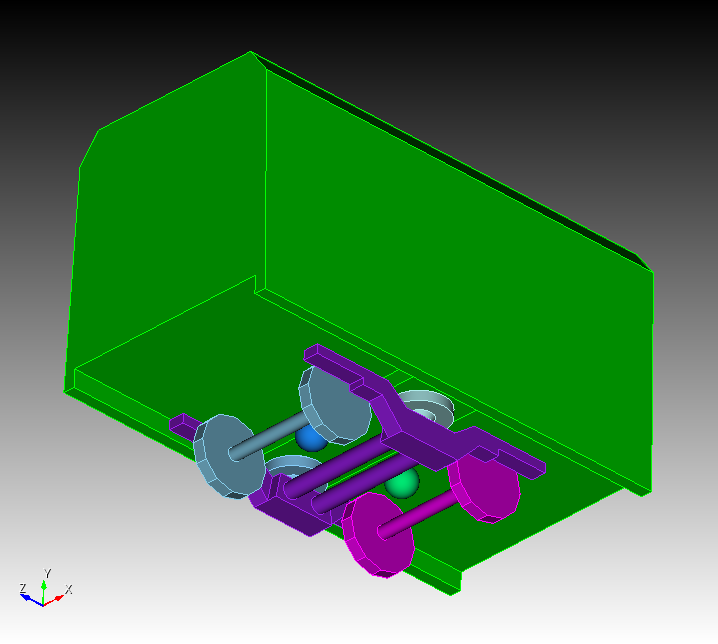
\includegraphics[width=\linewidth]{fig/chap4/geometry/initial_model_2.png}
		\caption{full model}
	\end{subfigure}
	\caption{Geometry of model}
\end{figure}



\subsection{Determination of simulation domain}
\subsection{Computational Effort}
The aim of this section is 

\section{Boundary conditions and loads}
\label{section:boundary_conditions}
\subsection{Modeling of sound source}

\section{General simulation setup}

\section{Parametric study}
\label{section:parametric_study}
\subsection{Variation of underfloor geometry}

\begin{figure}[H]
	\centering
	\begin{subfigure}[b]{0.49\textwidth}
		\centering
		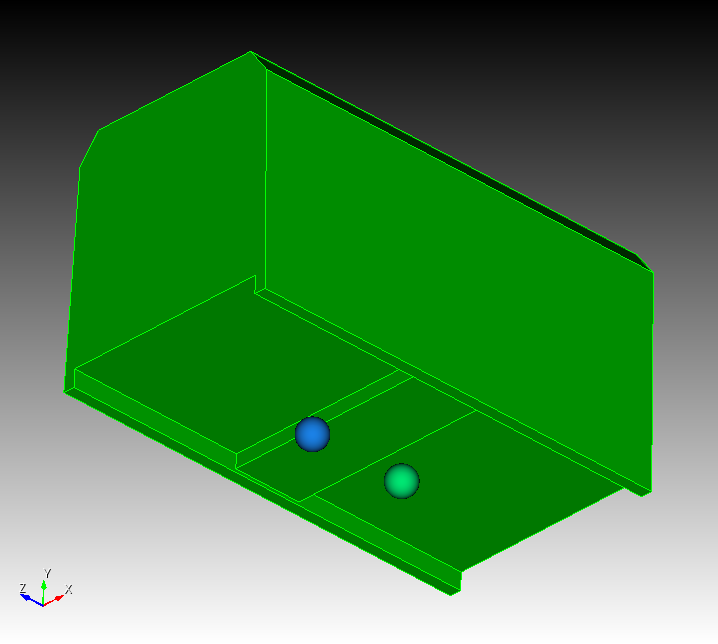
\includegraphics[width = 0.8\linewidth]{fig/chap4/geometry/no_underfloor_components_2.png}
		\caption{No underfloor components}
	\end{subfigure}
	\begin{subfigure}[b]{0.49\textwidth}
		\centering
		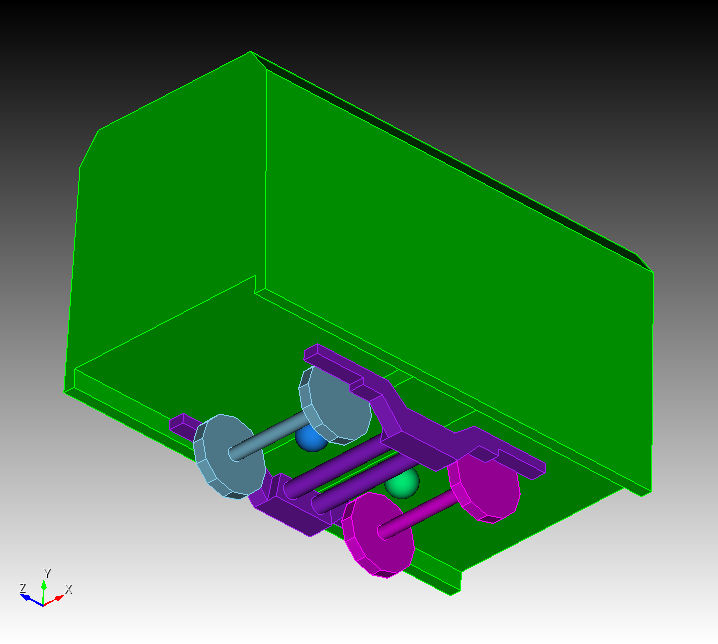
\includegraphics[width = 0.8\linewidth]{fig/chap4/geometry/no_air_suspension_2.png}
		\caption{No air suspension}
	\end{subfigure}
	\begin{subfigure}[b]{0.49\textwidth}
		\centering
		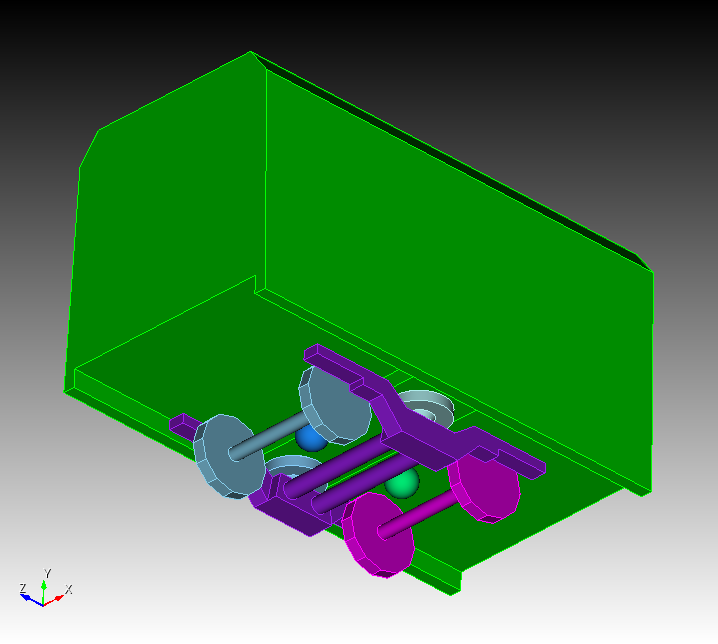
\includegraphics[width = 0.8\linewidth]{fig/chap4/geometry/initial_model_2.png}
		\caption{Initial model}
	\end{subfigure}
	\begin{subfigure}[b]{0.49\textwidth}
		\centering
		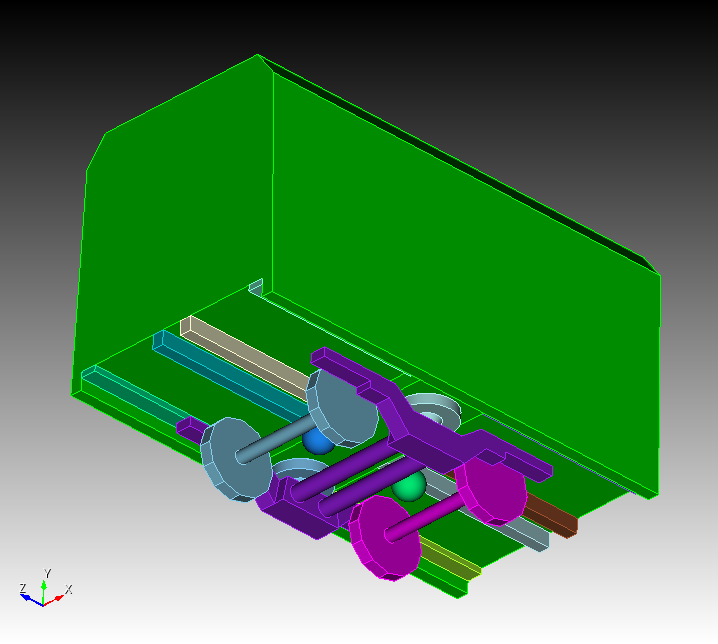
\includegraphics[width = 0.8\linewidth]{fig/chap4/geometry/additional_structures.png}
		\caption{Additional structures}
	\end{subfigure}

	\caption{Used geometry}
\end{figure}

\subsection{Inclusion of ground absorption}

\begin{figure}[H]
	\centering
	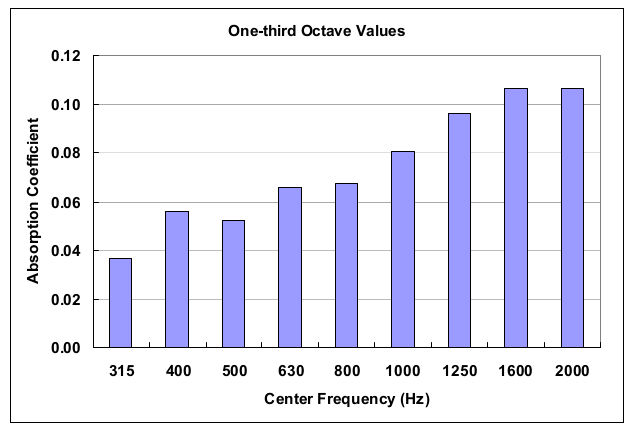
\includegraphics[width=0.7\textwidth]{fig/chap4/impedance/absorption_spectrum.png}
	\caption{Absorption coefficient in one-third octave bands \cite{Seybert2008MeasurementOP}}
	\label{fig:ground_absorption}
\end{figure}

\begin{table}[H]
	\caption{Estimated absorption coefficient from fig. \ref{fig:ground_absorption}, the values for frequency lower than 315 Hz are chosen arbitrary}
	\begin{tabular}{c|ccccccc}
		Freq (Hz)           & 100  & 125  & 160  & 200  & 250  & 315  & 400 \\ \hline
		$\alpha$ & 0.02 & 0.02 & 0.02 & 0.02 & 0.02 & 0.035 & 0.055
	\end{tabular}
	\newline
	\vspace*{10pt}
	\newline
	\begin{tabular}{c|ccccccc}
		Freq (Hz)  &  500  & 630  & 800  & 1000 & 1250 & 1600 & 2000 \\ \hline
		$\alpha$ & 0.05 & 0.065 & 0.065 & 0.08 & 0.095 & 0.105 & 0.105
	\end{tabular}
\end{table}

\begin{equation}
	\alpha = 1 - |r^2|
\end{equation}

\begin{equation}
	r = \frac{Z_s - Z_0}{Z_s + Z_0} = \frac{\frac{Z_s}{Z_0} - 1}{\frac{Z_s}{Z_0} + 1}
\end{equation}

\begin{equation}
	\tilde{Z_s} = \frac{Z_s}{Z_0} = \tilde{R} + j\tilde{X}
\end{equation}



\begin{equation}
	\begin{cases}
		\frac{4\tilde{R_s}}{\tilde{R_s}^2+\tilde{X_s}^2 + 2\tilde{R_s} + 1} = \alpha\\
		\arctan{\frac{\tilde{X_s}}{\tilde{R_s}}} = \varphi
	\end{cases}	
	\label{eq:impedance}
\end{equation}


\begin{figure}[H]
	\centering
	\begin{subfigure}[b]{0.8\textwidth}
		\centering
		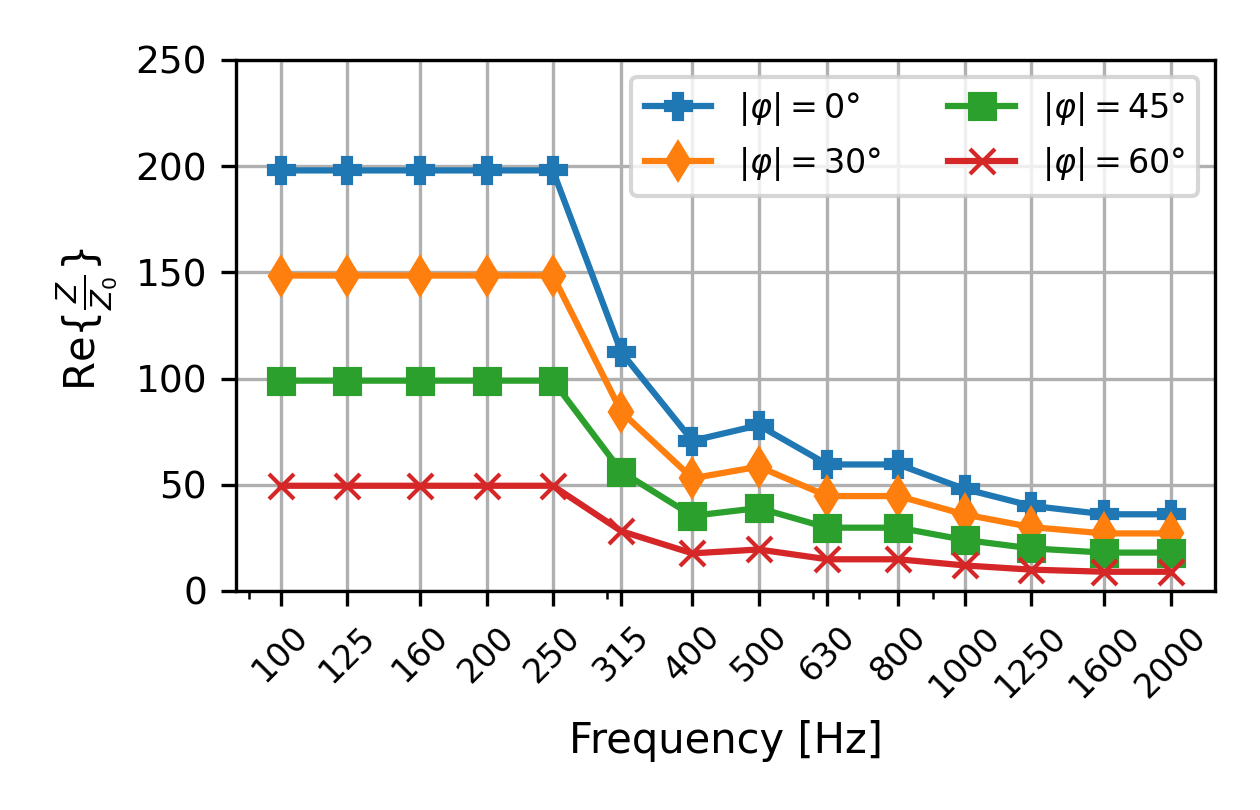
\includegraphics{fig/chap4/impedance/impedance_real.png}
	\end{subfigure}
	\begin{subfigure}[b]{0.8\textwidth}
		\centering
		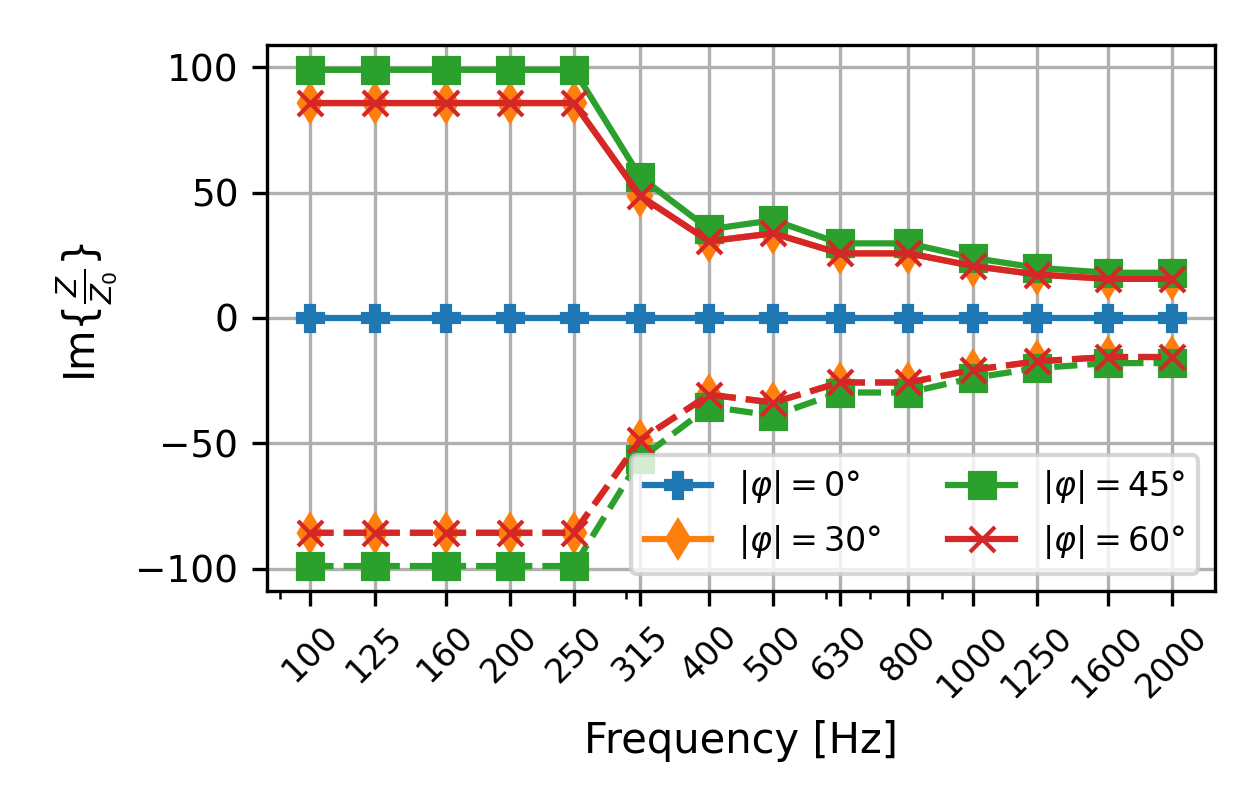
\includegraphics{fig/chap4/impedance/impedance_imag.png}
	\end{subfigure}
	\caption{Input impedance in one-third octave bands}
\end{figure}


\subsection{Variation of frequency steps per 1/3-octave band}